% ============================================================
\chapter{NumPy II: matrizes, sistemas lineares e polinômios}
\label{cap:aula5}
% ============================================================

\begin{objetivos}
\begin{itemize}
  \item criar matrizes como \emph{arrays} bidimensionais e acessar linhas, colunas e submatrizes;
  \item distinguir o produto elemento a elemento (\py{*}) do produto de matrizes (\py{@});
  \item calcular transposta, determinante, inversa, posto, autovalores e autovetores com \py{np.linalg};
  \item resolver sistemas lineares com \py{np.linalg.solve} e programar a eliminação de Gauss;
  \item trabalhar com polinômios: raízes, avaliação e ajuste de curvas (\py{np.roots}, \py{np.polyval}, \py{np.polyfit}).
\end{itemize}
\end{objetivos}

\begin{roteiro}
0--15 min & Matrizes no NumPy: criação, \py{shape}, índices, linhas, colunas, matrizes especiais.\\
15--30 min & Operações: soma, \py{*} \emph{versus} \py{@}, transposta, potências.\\
30--45 min & \py{np.linalg}: \py{det}, \py{inv}, \py{solve}, \texttt{matrix\_rank}; sistemas lineares.\\
45--60 min & Eliminação de Gauss programada (exercício do livro da SBM).\\
60--75 min & Autovalores e autovetores; polinômios e ajuste por mínimos quadrados.\\
75--90 min & Exercícios.\\
\end{roteiro}

% ------------------------------------------------------------
\section{Matrizes como \emph{arrays} bidimensionais}
% ------------------------------------------------------------

Uma matriz é criada a partir de uma lista de linhas:

\begin{entrada}
import numpy as np
A = np.array([[1, 2, 3],
              [4, 5, 6]])
print(A)
print("forma:", A.shape, " elementos:", A.size, " dimensões:", A.ndim)
\end{entrada}
\begin{saida}
[[1 2 3]
 [4 5 6]]
forma: (2, 3)  elementos: 6  dimensões: 2
\end{saida}

O elemento da linha $i$ e coluna $j$ é \py{A[i, j]} (contando a partir de 0). O símbolo \py{:} sozinho
significa ``todos'': \py{A[i, :]} é a linha $i$ e \py{A[:, j]} é a coluna $j$.

\begin{figure}[ht]
\centering
\begin{tikzpicture}[font=\ttfamily\small, cel/.style={draw=gray!60, minimum size=0.8cm}]
  \newcommand{\matriz}[3]{%
    \begin{scope}[shift={(#1,0)}]
    \foreach \v [count=\k from 0] in {1,2,3,4,5,6,7,8,9} {
       \pgfmathtruncatemacro{\i}{\k/3} \pgfmathtruncatemacro{\j}{mod(\k,3)}
       \node[cel] at (\j*0.8, -\i*0.8) {\v};
    }
    #2
    \node[font=\ttfamily] at (0.8,-2.7) {#3};
    \end{scope}}
  \matriz{0}{\draw[azul, very thick, fill=azul, fill opacity=0.15] (-0.4,-0.4) rectangle (2.0,-1.2);}{M[1, :]}
  \matriz{3.4}{\draw[verde, very thick, fill=verde, fill opacity=0.15] (1.2,0.4) rectangle (2.0,-2.0);}{M[:, 2]}
  \matriz{6.8}{\draw[vermelho, very thick, fill=vermelho, fill opacity=0.15] (-0.4,0.4) rectangle (1.2,-1.2);}{M[:2, :2]}
  \matriz{10.2}{\draw[laranja, very thick, fill=laranja, fill opacity=0.15] (0.4,-0.4) rectangle (1.2,-1.2);}{M[1, 1]}
\end{tikzpicture}
\caption{Seleção de linha, coluna, submatriz e elemento em \texttt{M = np.arange(1, 10).reshape(3, 3)}.}
\label{fig:fatias-matriz}
\end{figure}

\begin{entrada}
M = np.arange(1, 10).reshape(3, 3)   # 1..9 arrumados em 3 x 3
print(M)
print(M[1, 1], M[0, 2], M[-1, -1])
print(M[1, :], M[:, 2])
print(M[:2, :2])
\end{entrada}
\begin{saida}
[[1 2 3]
 [4 5 6]
 [7 8 9]]
5 3 9
[4 5 6] [3 6 9]
[[1 2]
 [4 5]]
\end{saida}

\begin{maxima}
No Maxima: \texttt{M: matrix([1,2,3],[4,5,6],[7,8,9])}, o elemento é \texttt{M[2,2]} (contando a partir de 1),
a linha é \texttt{row(M,2)} e a coluna \texttt{col(M,3)}. No NumPy a contagem começa em 0: \py{M[1, 1]},
\py{M[1, :]}, \py{M[:, 2]}.
\end{maxima}

\paragraph{Matrizes especiais.}

\begin{entrada}
print(np.eye(3))                  # identidade
print(np.zeros((2, 3)))           # nula 2 x 3 (note os parênteses duplos)
print(np.diag([1, 2, 3]))         # diagonal
print(np.ones((2, 2), dtype=int))
\end{entrada}
\begin{saida}
[[1. 0. 0.]
 [0. 1. 0.]
 [0. 0. 1.]]
[[0. 0. 0.]
 [0. 0. 0.]]
[[1 0 0]
 [0 2 0]
 [0 0 3]]
[[1 1]
 [1 1]]
\end{saida}

Também podemos construir uma matriz a partir de uma fórmula para $a_{ij}$. Por exemplo, a matriz de Hilbert
$h_{ij}=\frac{1}{i+j-1}$ (com $i,j$ começando em 1):

\begin{entrada}
n = 4
i = np.arange(1, n + 1).reshape(n, 1)    # coluna
j = np.arange(1, n + 1).reshape(1, n)    # linha
H = 1 / (i + j - 1)                      # "broadcasting": vira n x n
print(np.round(H, 4))
\end{entrada}
\begin{saida}
[[1.     0.5    0.3333 0.25  ]
 [0.5    0.3333 0.25   0.2   ]
 [0.3333 0.25   0.2    0.1667]
 [0.25   0.2    0.1667 0.1429]]
\end{saida}

% ------------------------------------------------------------
\section{Operações com matrizes}
% ------------------------------------------------------------

\begin{center}
\begin{tabular}{@{}lll@{}}
\toprule
\textbf{Matemática} & \textbf{NumPy} & \textbf{Observação}\\
\midrule
$A+B$, $A-B$, $kA$ & \py{A + B}, \py{A - B}, \py{k * A} & \\
$AB$ (produto de matrizes) & \py{A @ B} ou \py{np.dot(A, B)} & \textbf{não} é \py{A * B}\\
$A^T$ & \py{A.T} ou \py{np.transpose(A)} & \\
$A^n$ & \py{np.linalg.matrix_power(A, n)} & \textbf{não} é \py{A**n}\\
$\det A$ & \py{np.linalg.det(A)} & resultado aproximado\\
$A^{-1}$ & \py{np.linalg.inv(A)} & \\
$\operatorname{posto}(A)$ & \py{np.linalg.matrix_rank(A)} & \\
$\operatorname{tr}(A)$ & \py{np.trace(A)} & \\
solução de $Ax=b$ & \py{np.linalg.solve(A, b)} & $A$ quadrada e invertível\\
autovalores/autovetores & \py{np.linalg.eig(A)} & \\
\bottomrule
\end{tabular}
\end{center}

\begin{entrada}
A = np.array([[1, 2], [-3, 1]])
B = np.array([[2, 5], [4, 10]])
print("A * B =\n", A * B)      # elemento a elemento
print("A @ B =\n", A @ B)      # produto de matrizes
print("B @ A =\n", B @ A)      # em geral AB != BA
print("A^T =\n", A.T)
\end{entrada}
\begin{saida}
A * B =
 [[  2  10]
 [-12  10]]
A @ B =
 [[10 25]
 [-2 -5]]
B @ A =
 [[-13   9]
 [-26  18]]
A^T =
 [[ 1 -3]
 [ 2  1]]
\end{saida}

\begin{atencao}
\py{A * B} e \py{A ** 2} operam \textbf{elemento a elemento}. Para o produto matricial use \py{A @ B}; para
potências, \py{A @ A} ou \py{np.linalg.matrix_power(A, n)}. Multiplicar matrizes de tamanhos incompatíveis
gera \py{ValueError}.
\end{atencao}

\begin{entrada}
print(np.linalg.det(A), np.linalg.det(B))
Ainv = np.linalg.inv(A)
print(Ainv)
print(A @ Ainv)
print(np.allclose(A @ Ainv, np.eye(2)))
\end{entrada}
\begin{saida}
7.000000000000001 0.0
[[ 0.14285714 -0.28571429]
 [ 0.42857143  0.14285714]]
[[1. 0.]
 [0. 1.]]
True
\end{saida}

Note o pequeno erro de arredondamento: $\det A=7$, mas apareceu \py{7.000000000000001}. Erros desse tipo
(da ordem de $10^{-16}$) podem aparecer em qualquer conta com \py{float}; por isso, para comparar matrizes,
usa-se \py{np.allclose}, que admite uma pequena tolerância. Os cálculos \emph{exatos} (como no Maxima) serão feitos com o SymPy na Aula 10.

% erro
\begin{entrada}
np.linalg.inv(B)            # det(B) = 0
\end{entrada}
\begin{saida}
LinAlgError: Singular matrix
\end{saida}

\paragraph{Exemplo: Fibonacci por potências de matriz.} Como
$\begin{pmatrix}F_{n+1}\\F_n\end{pmatrix}=\begin{pmatrix}1&1\\1&0\end{pmatrix}\begin{pmatrix}F_{n}\\F_{n-1}\end{pmatrix}$,
temos $\begin{pmatrix}1&1\\1&0\end{pmatrix}^n=\begin{pmatrix}F_{n+1}&F_n\\F_n&F_{n-1}\end{pmatrix}$.

\begin{entrada}
Q = np.array([[1, 1], [1, 0]])
print(np.linalg.matrix_power(Q, 10))
\end{entrada}
\begin{saida}
[[89 55]
 [55 34]]
\end{saida}

% ------------------------------------------------------------
\section{Sistemas lineares}
% ------------------------------------------------------------

O sistema
\[
\begin{cases} x_0+2x_1=1\\ 3x_0+5x_1=2\end{cases}
\qquad\Longleftrightarrow\qquad
\underbrace{\begin{pmatrix}1&2\\3&5\end{pmatrix}}_{A}\begin{pmatrix}x_0\\x_1\end{pmatrix}=\underbrace{\begin{pmatrix}1\\2\end{pmatrix}}_{b}
\]
(exemplo do livro da SBM) se resolve com \py{np.linalg.solve(A, b)}. Geometricamente, a solução é o ponto de
encontro das duas retas (Figura~\ref{fig:retas}).

\begin{figure}[ht]
\centering
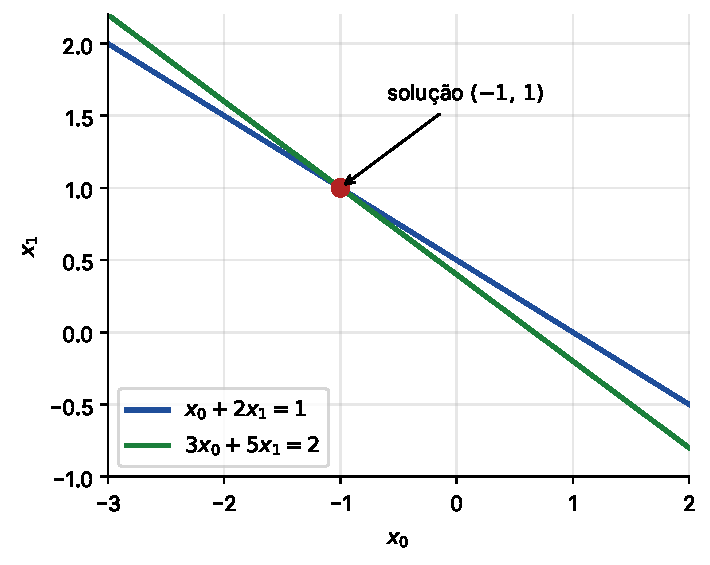
\includegraphics[width=0.55\linewidth]{aula05-retas}
\caption{As retas $x_0+2x_1=1$ e $3x_0+5x_1=2$ se encontram em $(-1,1)$.}
\label{fig:retas}
\end{figure}

\begin{entrada}
A = np.array([[1, 2], [3, 5]])
b = np.array([1, 2])
x = np.linalg.solve(A, b)
print(x)
print(np.allclose(A @ x, b))        # verificação: Ax = b ?
\end{entrada}
\begin{saida}
[-1.  1.]
True
\end{saida}

Um sistema $3\times3$:
\[
\begin{cases} x+y-2z=1\\ x+y-z=3\\ 3x+y-z=3 \end{cases}
\]

\begin{entrada}
A = np.array([[1, 1, -2], [1, 1, -1], [3, 1, -1]])
b = np.array([1, 3, 3])
print(np.linalg.det(A))
print(np.linalg.solve(A, b))
\end{entrada}
\begin{saida}
2.0000000000000004
[0. 5. 2.]
\end{saida}

\begin{observacao}
\py{np.linalg.solve} só funciona para matrizes quadradas invertíveis. Se o sistema for impossível ou
indeterminado ($\det A=0$), ele gera \py{LinAlgError}. Para analisar esses casos, compare o posto da matriz dos
coeficientes com o da matriz ampliada (Teorema de Rouché--Capelli), usando \py{np.linalg.matrix_rank}, ou use o
SymPy (Aula 10).
\end{observacao}

\begin{entrada}
A = np.array([[1, 2], [2, 4]])
for b in [np.array([3, 6]), np.array([3, 7])]:
    Ab = np.column_stack([A, b])            # matriz ampliada [A | b]
    print(b, np.linalg.matrix_rank(A), np.linalg.matrix_rank(Ab))
\end{entrada}
\begin{saida}
[3 6] 1 1
[3 7] 1 2
\end{saida}

No primeiro caso os postos são iguais (1) e menores que o número de incógnitas: sistema possível e
indeterminado. No segundo, os postos diferem: sistema impossível.

% ------------------------------------------------------------
\section{Programando a eliminação de Gauss}
% ------------------------------------------------------------

O livro da SBM (Exemplo 3.35 e Exercício 3) propõe programar o método de eliminação de Gauss. Com o NumPy as
operações com linhas ficam bem mais simples, pois \py{M[i]} é a linha $i$ inteira e podemos fazer
\py{M[j] = M[j] - fator * M[i]}.

O método tem duas etapas:
\begin{enumerate}
  \item \textbf{Escalonamento}: para cada coluna $i$, escolhe-se como pivô o elemento de maior módulo na coluna
  (da linha $i$ para baixo), troca-se a sua linha com a linha $i$, e zeram-se os elementos abaixo do pivô com
  $L_j \leftarrow L_j - \frac{a_{ji}}{a_{ii}}L_i$.
  \item \textbf{Retrossubstituição}: no sistema triangular $Ux=c$, calcula-se $x_{n-1}$, depois $x_{n-2}$, e assim
  por diante: $x_i=\dfrac{c_i-\sum_{j>i}u_{ij}x_j}{u_{ii}}$.
\end{enumerate}

\begin{entrada}
def escalona(A, b):
    """Escalona a matriz ampliada [A | b] (com pivoteamento parcial)."""
    M = np.column_stack([A, b]).astype(float)
    n = len(b)
    for i in range(n - 1):
        p = i + np.argmax(np.abs(M[i:, i]))   # linha do maior pivô
        if M[p, i] == 0:
            raise ValueError("matriz singular")
        M[[i, p]] = M[[p, i]]                 # troca as linhas i e p
        for j in range(i + 1, n):
            fator = M[j, i] / M[i, i]
            M[j] = M[j] - fator * M[i]
    return M

def retrossubstituicao(M):
    n = M.shape[0]
    x = np.zeros(n)
    for i in range(n - 1, -1, -1):            # i = n-1, ..., 1, 0
        x[i] = (M[i, -1] - M[i, i+1:n] @ x[i+1:]) / M[i, i]
    return x

def gauss(A, b):
    return retrossubstituicao(escalona(A, b))
\end{entrada}

Vamos testar com o sistema do livro da SBM, cuja matriz ampliada é
\[
\left(\begin{array}{rrrr|r}
1 & -1 & 2 & -1 & -8\\
2 & -2 & 3 & -3 & -20\\
1 & 1 & 1 & 0 & -2\\
1 & -1 & 4 & -3 & 4
\end{array}\right).
\]
Repare que, depois do primeiro passo, aparece um zero na posição do segundo pivô: sem a troca de linhas o método
falharia.

\begin{entrada}
A = np.array([[1, -1, 2, -1], [2, -2, 3, -3], [1, 1, 1, 0], [1, -1, 4, -3]])
b = np.array([-8, -20, -2, 4])
np.set_printoptions(precision=3, suppress=True)
print(escalona(A, b))
x = gauss(A, b)
print("x =", x)
print("conferindo com solve:", np.linalg.solve(A, b))
\end{entrada}
\begin{saida}
[[  2.   -2.    3.   -3.  -20. ]
 [  0.    2.   -0.5   1.5   8. ]
 [  0.    0.    2.5  -1.5  14. ]
 [  0.    0.    0.    0.8  -0.8]]
x = [-13.   6.   5.  -1.]
conferindo com solve: [-13.   6.   5.  -1.]
\end{saida}

\begin{observacao}
O comando \py{np.set_printoptions(precision=3, suppress=True)} faz o NumPy mostrar 3 casas decimais e não usar
notação científica para números muito pequenos. Ele vale para o resto do notebook; para voltar ao padrão, use
\py{np.set_printoptions(precision=8, suppress=False)}.
\end{observacao}

% ------------------------------------------------------------
\section{Autovalores e autovetores}
% ------------------------------------------------------------

Um número $\lambda$ é autovalor de $A$ se existe $v\neq0$ com $Av=\lambda v$. O comando \py{np.linalg.eig(A)}
devolve os autovalores e uma matriz cujas \textbf{colunas} são autovetores (normalizados, com norma 1). Para
matrizes \textbf{simétricas} há o \py{np.linalg.eigh}, que devolve os autovalores reais e em ordem crescente.

\begin{entrada}
A = np.array([[2, 1], [1, 2]])
autovalores, V = np.linalg.eigh(A)     # A é simétrica
print(autovalores)
print(V)
v = V[:, 1]                          # autovetor da coluna 1 (lambda = 3)
print(A @ v, autovalores[1] * v)     # A v = lambda v
\end{entrada}
\begin{saida}
[1. 3.]
[[-0.707  0.707]
 [ 0.707  0.707]]
[2.121 2.121] [2.121 2.121]
\end{saida}

\begin{figure}[ht]
\centering
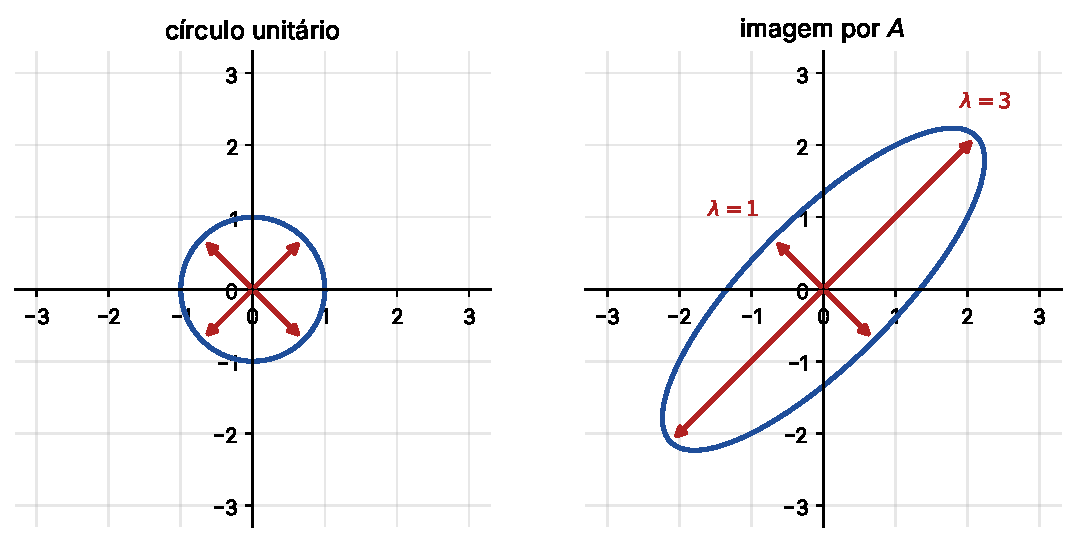
\includegraphics[width=0.8\linewidth]{aula05-transformacao}
\caption{A matriz $A=\begin{pmatrix}2&1\\1&2\end{pmatrix}$ transforma o círculo unitário em uma elipse. Os
autovetores (em vermelho) são as direções que não giram: são apenas esticadas, pelos fatores $\lambda=3$ e $\lambda=1$.}
\end{figure}

Para uma matriz de rotação de $90^\circ$ nenhuma direção é preservada, e os autovalores são complexos:

\begin{entrada}
R = np.array([[0, -1], [1, 0]])
print(np.linalg.eig(R)[0])
\end{entrada}
\begin{saida}
[0.+1.j 0.-1.j]
\end{saida}

% ------------------------------------------------------------
\section{Polinômios}
% ------------------------------------------------------------

No NumPy, um polinômio é representado pela lista de coeficientes, \textbf{do maior grau para o menor}:
$p(x)=x^3-6x^2+11x-6$ é \py{[1, -6, 11, -6]}.

\begin{entrada}
p = [1, -6, 11, -6]
print(np.roots(p))                    # raízes
print(np.polyval(p, [0, 1, 4]))       # p(0), p(1), p(4)
print(np.roots([1, 0, 1]))            # x^2 + 1: raízes complexas
print(np.poly([1, 2, 3]))             # polinômio com raízes 1, 2, 3
\end{entrada}
\begin{saida}
[3. 2. 1.]
[-6  0  6]
[-0.+1.j  0.-1.j]
[ 1. -6. 11. -6.]
\end{saida}

\paragraph{Ajuste de curvas (mínimos quadrados).} Dados pontos $(x_i,y_i)$ experimentais, \py{np.polyfit(x, y, grau)}
encontra o polinômio do grau pedido que melhor se ajusta aos dados (minimizando $\sum (p(x_i)-y_i)^2$).

\begin{entrada}
x = np.array([0, 1, 2, 3, 4, 5])
y = np.array([1.1, 2.9, 5.2, 7.1, 8.8, 11.2])
a, b = np.polyfit(x, y, 1)            # reta y = a x + b
print(f"y = {a:.3f} x + {b:.3f}")
print(f"previsão para x = 6: {np.polyval([a, b], 6):.2f}")
\end{entrada}
\begin{saida}
y = 2.003 x + 1.043
previsão para x = 6: 13.06
\end{saida}

O gráfico desses dados com a reta ajustada é feito na Aula~6.

\begin{professor}
Se a turma já viu escalonamento em Álgebra Linear, vale fazer o primeiro passo da eliminação no quadro e comparar
com a saída de \texttt{escalona}. A função usa \texttt{M[[i, p]] = M[[p, i]]} para trocar linhas, um recurso
(``indexação por lista'') que pode precisar de explicação.
\end{professor}

% ------------------------------------------------------------
\section{Exercícios}
% ------------------------------------------------------------

\begin{exercicio}[operações]{ex:5-ops}
Sejam $A=\begin{pmatrix}1&2&0\\0&1&3\\4&0&1\end{pmatrix}$ e $B=\begin{pmatrix}2&0&1\\1&1&0\\0&3&1\end{pmatrix}$.
Calcule $A+B$, $AB$, $BA$, $A^TB$, $\det(AB)$ e $\det A\cdot\det B$. Verifique que $(AB)^T=B^TA^T$.
\end{exercicio}

\begin{exercicio}[sistema]{ex:5-sistema}
Resolva com \py{np.linalg.solve} e com a função \py{gauss}:
$\begin{cases}2x+y-z=8\\-3x-y+2z=-11\\-2x+y+2z=-3\end{cases}$.
\end{exercicio}

\begin{exercicio}[matriz de Hilbert]{ex:5-hilbert}
Para $n=4, 8, 12$, crie a matriz de Hilbert $H_n$, tome $x=(1,1,\dots,1)$, calcule $b=H_nx$ e resolva $H_ny=b$.
Compare $y$ com $x$. O que acontece? (Pesquise ``matriz mal condicionada'' e use \py{np.linalg.cond}.)
\end{exercicio}

\begin{exercicio}[autovalores]{ex:5-autov}
Calcule os autovalores e autovetores de $\begin{pmatrix}4&1\\2&3\end{pmatrix}$ e verifique $Av=\lambda v$ para cada par.
Confira que a soma dos autovalores é o traço e o produto é o determinante.
\end{exercicio}

\begin{exercicio}[polinômios]{ex:5-poli}
Encontre as raízes de $x^4-5x^2+4$ e de $x^3-2x-5$. Use \py{np.polyval} para conferir que são raízes.
\end{exercicio}

\begin{exercicio}[extra: ajuste de parábola]{ex:5-ajuste}
Um objeto é lançado e sua altura (m) é medida nos instantes $t=0, 0{,}5, 1, 1{,}5, 2, 2{,}5$\,s:
$h=1{,}0;\ 7{,}9;\ 12{,}4;\ 14{,}6;\ 14{,}3;\ 11{,}7$. Ajuste uma parábola $h(t)=at^2+bt+c$ e estime a aceleração da
gravidade ($g\approx-2a$) e o instante de altura máxima.
\end{exercicio}
